
\documentclass[a4paper]{article}

\usepackage[T2A]{fontenc}
\usepackage[russian]{babel}
\usepackage{graphicx}
\usepackage{float}
\usepackage{hyperref}
\usepackage{amsmath, amssymb}
\usepackage{caption}
\usepackage{geometry}
\usepackage{pdfpages}
\geometry{top=2cm,bottom=2cm,left=2cm,right=2cm}

\newcommand{\minus}{\scalebox{0.75}[1.0]{$-$}}


\date{}

\begin{document}

\begin{center}
\textsc{Санкт-Петербургский национальный исследовательский институт информационных технологий, механики и оптики\\[3mm]
Физический факультет} \\[3mm]

\end{center}
\vspace{5mm}
\line(1,0){\textwidth}
\begin{center}
\textbf{ЛАБОРАТОРНАЯ РАБОТА №1.11\\}
\textbf{"Измерение ускорения свободного падения с помощью оборотного маятника"}
\end{center}
\vspace{2mm}
\line(1,0){\textwidth}
\vspace{5mm}
\begin{minipage}{0.4\textwidth}
    Группа: Z3144 \\
    Студент: Евгений Турчанин\\
    \vspace{1mm}
\end{minipage}
\hfill
\vspace{1mm}
\line(1,0){\textwidth}

\section{\textbf{Цели работы}}
\begin{enumerate}
	\item Экспериментальная проверка закономерностей движения физического маятника.
\end{enumerate}

\section {\textbf{Задачи}}
\begin{enumerate}
	\item Определение периода колебаний маятника при совпадении приведенной длины с расстоянием между призмами.
	\item Определение ускорения свободного падения с абсолютной и относительной погрешностями.
	\item Сравнение найденного ускорения свободного падения со справочным значением для широты лаборатории.
\end{enumerate}


\section{\text{Теорическое введение}}

Физическим маятником называется твердое тело, имеющее возможность совершать колебания под действием силы тяжести вокруг неподвижной горизонтальной оси (рис. 1)
\begin{figure}[H]
\center{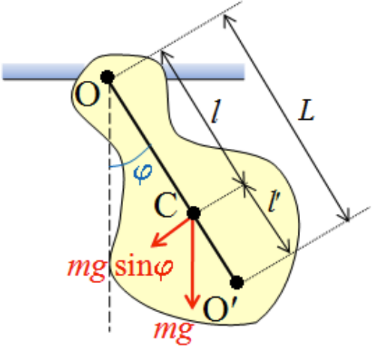
\includegraphics[scale=0.8]{1}}
\caption{Физический маятник.O - точка подвеса, С - центр инерции,$O'$- центр качания.}
\end{figure}
Обозначим расстояние от точки подвеса до центра инерции
как $l$, возвращающий момент по-прежнему будет равен
$M=-mgl\varphi$ (при малых углах отклонения), но второй закон Ньютона теперь запишется в виде:
\begin{equation}
mgl\varphi=-I\ddot{\varphi}
\end{equation}
где $I$ – момент инерции маятника относительно оси подвеса,
который зависит от распределения масс.\\
Соответственно период малых колебаний физического маятника равен
\begin{equation}
T=2\pi\sqrt{\dfrac{I}{mgl}}
\end{equation}
Соотношение (2) удобно преобразовать, используя теорему
Штейнера:
\begin{equation}
I=I_0+ml^2
\end{equation}
где $I_0$ – момент инерции маятника относительно оси, проходящей
через его центр инерции параллельно оси подвеса. Тогда для
периода колебаний получаем:

\begin{equation}
T=2\pi\sqrt{\dfrac{I_0+ml^2}{mgl}}
\end{equation}

Проанализируем зависимость $T(l)$. График этой функции приведен на рис. 2.
\begin{figure}[H]
\center{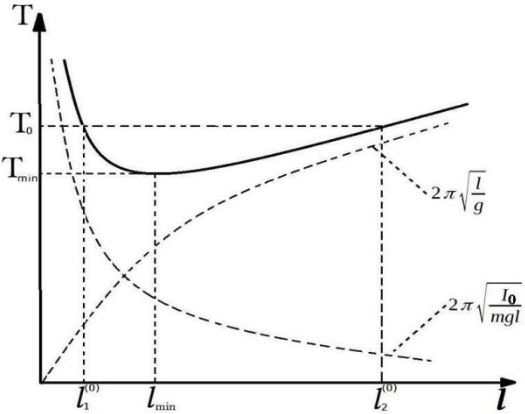
\includegraphics[scale=0.6]{2}}
\caption{Зависимость периода колебаний физического маятника от расстояния от оси подвеса до центра масс.}
\end{figure}


При малых $l$ маятник близок к положению безразличного
равновесия. В этом случае из (4) получаем:

\begin{equation}
	T(l)_{l\rightarrow0}=2\pi\sqrt{\dfrac{I_0}{mgl}}\rightarrow \infty
\end{equation}


В отличие от математического маятника, период колебаний
физического маятника при уменьшении длины тоже растет.\\
Взяв производную от правой части (4) и приравняв ее нулю,
найдем, что минимальный период колебаний физического маятника получается при
$l_{min}=\sqrt{\dfrac{I_0}{m}}$ и равен:

\begin{equation}
	T_{min}=2\pi\sqrt{\dfrac{2}{g}\sqrt{\dfrac{I_0}{m}}}
\end{equation}

Рассмотрим математический маятник, имеющий такой же период колебаний, как и физический. Очевидно, что его длина
должна быть:

\begin{equation}
	L=\dfrac{I}{ml}=\dfrac{I_0}{ml}+l
\end{equation}
Величина $L$ называется приведенной длиной физического маятника. Точка на прямой, соединяющей точку подвеса с центром
инерции, лежащая на расстоянии $L$ от точки подвеса, называется центром качания физического маятника (точка $O'$ на рис. 1).\\
Из (7) видно, что $L>l$, следовательно, точка подвеса и центр
качания лежат по разные стороны от центра инерции.
Если перевернуть физический маятник и подвесить его в точке, совпадающей с центром качания, то новое расстояние до центра инерции будет равно $l'=L-l$ (рис. 1).\\ Нетрудно доказать,
что приведенная длина, а значит и период колебания при этом не
изменятся. Следовательно, при переносе точки подвеса в центр
качания прежняя точка подвеса становится новым центром качания\\
Графически это свойство иллюстрирует рис. 2. Из него следует, что один и тот же период колебаний физического маятника
$T_0$ реализуется при двух значениях $l=l_{01} и l'=l_{02}$.\\

\textbf{Оборотный маятник}
Рассмотренное свойство физического маятника можно использовать для измерения ускорения свободного падения. Заметим,
что недостаточно просто измерить период колебания маятника,
т.к. в расчетные формулы входят трудноопределимые величины момента инерции и расстояния до центра инерции. Поэтому
используют специальный вариант физического маятника, называемый оборотным (рис. 3).

Маятник состоит из металлического стержня 1, на котором
закреплены массивные грузы 4 и 5. Осями подвеса служат ребра двух призм 2, закрепленных вблизи концов стержня. Расстояние между призмами фиксировано. В рабочем положении призмы
устанавливаются в $V$-образные опоры 3. Центр инерции маятника находится где-то между призмами.
Регулируемым параметром является положение груза 4. Очевидно, что при перемещении этого груза в направлении призмы 2
центр инерции будет смещаться вниз, увеличивая расстояние $l$ от
точки подвеса. Если же маятник перевернуть, то такое же смещение регулировочного груза приведет к поднятию центра инерции
и уменьшению $l$. В обоих случаях меняются периоды колебаний
$T_1$ и $T_2$.
Если при каком-то положении регулировочного груза окажется, что $T_1=T_2=T_0$, то это будет означать, что вторая призма
находится в центре качания, а расстояние между призмами (которое легко измерить) равно приведенной длине маятника.\\
Измерив$T_0$, находим ускорение свободного падения
\[
g=\dfrac{4\pi^2L}{T_0^2}
\]
\begin{figure}[H]
\center{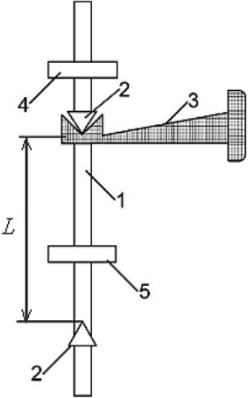
\includegraphics[scale=0.6]{3}}
\caption{Оборотный маятник.}
\end{figure}
\section{\text{Экспериментальная установка}}
Экспериментальная установка показана на рис. 4.
\begin{figure}[H]
\center{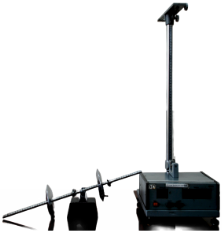
\includegraphics[scale=0.6]{4}}
\caption{Экспериментальная установка.}
\end{figure}

Основой установки служит оборотный маятник, схема которого приведена на рис. 3. Для измерения расстояния между призмами и положения регулировочного груза на стержне нанесены
риски с шагом 1 см.\\
Измерение времени колебаний производится электронным секундомером. При нажатии клавиши «СБРОС» начинается отсчет
времени с момента прохождения маятником положения равновесия. При нажатии клавиши «СТОП» секундомер выключается
после завершения текущего периода колебаний, индикатор показывает целое число периодов колебаний $N$ и время $t$, за которое
маятник их совершил.
\section{\text{Полученные данные}}
\begin{figure}[H]
\center{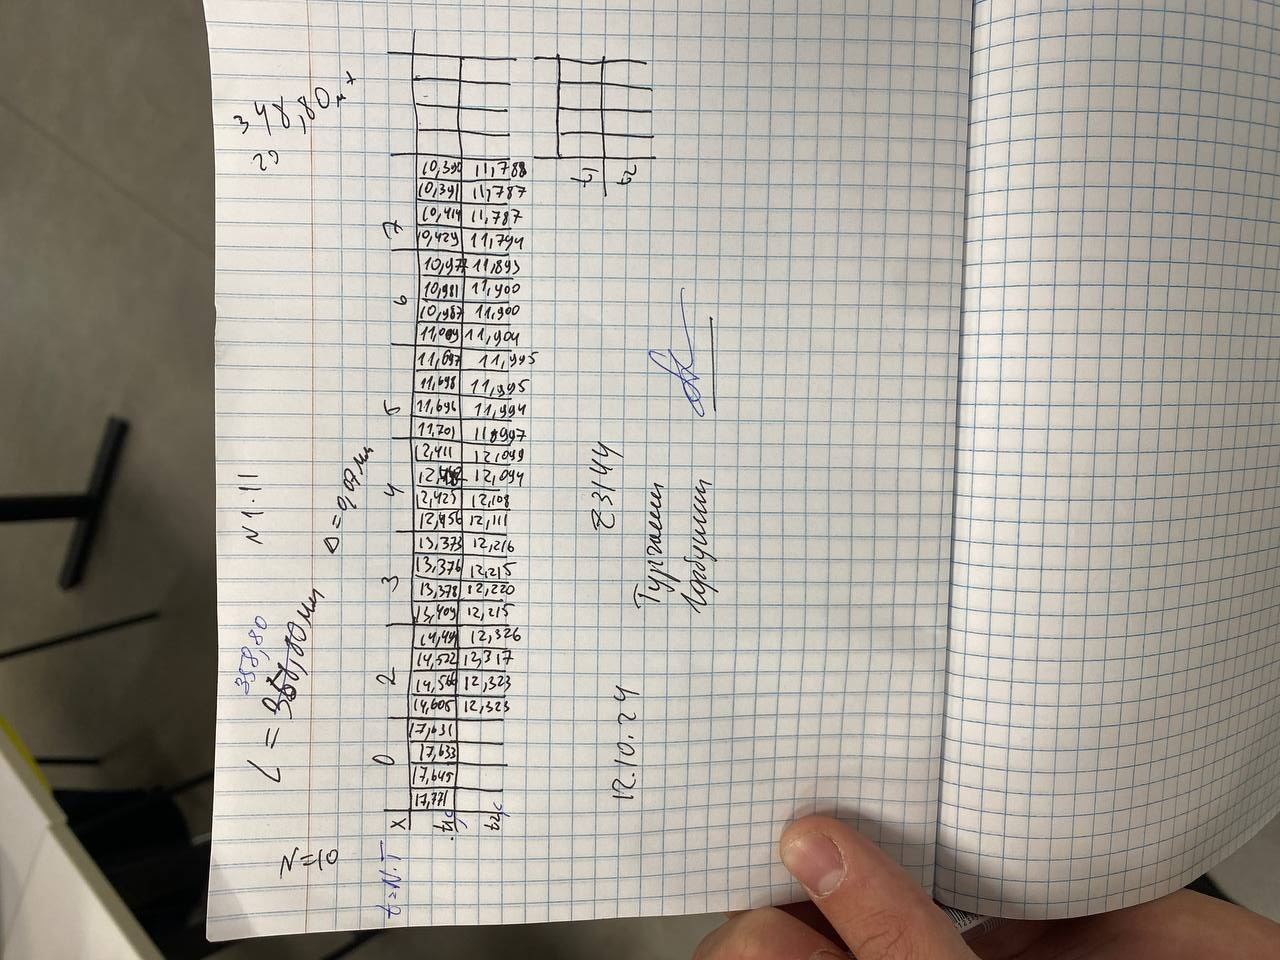
\includegraphics[scale=0.3]{lab_data.png}}
\caption{Полученные данные.}
\end{figure}



\section{\text{Результаты}}

Используя python обрабатываем данные и получаем:
\begin{figure}[H]
\center{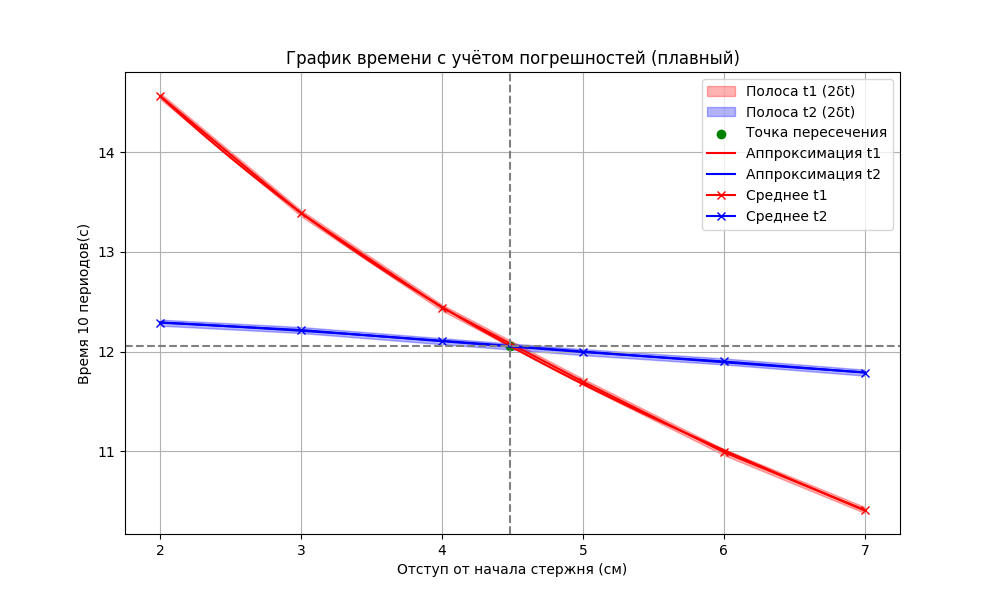
\includegraphics[scale=0.5]{Figure_1.png}}
\caption{Графики зависимостей $T_1(x)$ и $T_2(x)$}
\end{figure}
\begin{center}
Период 10 колебаний $T_0=12.058$с\\
Ускорение свободного падения: $g=9.8244$м/с$^2$\\
Относительная погрешность: $0.002414$\\
Абсолютная погрешность: $0.0237$
\end{center}
Абсолютное и относительное отклонения измеренного ускорения свободного падения от справочного значения для широты
лаборатории:\\
\begin{center}
Относительная погрешность: $0.0005$\\
Абсолютная погрешность: $-0.0049$
\end{center}
\section{\text{Заключение}}
Из приведенных выше данных можно сделать вывод, что ускорение свободного падения соответствует действительности, те эксперимент подтвердил справедливость теоретических зависимостей для физического маятник. Небольшие отклонения могут быть вызваны неточностью приборов.

\end{document}
